\clearpage
\section{Introduction}

In the Netherlands, public infrastructure maintainers (the state, provinces, municipalities and water authorities) have the legal responsibility for maintaining their assets. Maintaining the road means "to ensure that all roads within the area are in good condition" \cite{Wegenwet} . In this sense road maintainers are obliged to maintain facilities regularly and sustainable \cite{BurgerlijkWetbook6:174}. In order to give some guidance on how to assess the state of roads, standards are made by the national knowledge platform CROW. Among it activities the CROW prescribes road maintainers how to perform and assess road inspections \cite{CROW_147}. CROW helps maintainers in quality-driven management. 

Road maintenance is a big expenditure of the state's budget, it is annually around 2.5 - 3.5 billion (x1.000.000.000) EUR \cite{Rijksbegroting:Infrastructuur}. Depending on the type of the road, a different public body is responsible for maintaining that road. For instance, highways (indicated with A) are maintained by the state (Rijkswaterstaat), provincial (indicated with N) roads by the provinces, and local roads (indicated with street names) by municipalities. Public bodies are legally obliged to report "maintenance capital goods" in their annual budgets \cite{Wet_Besluit_Begroting}. Within the report they have to state the policy framework for maintenance and the financial implications. From this, it flows that road maintenance is planned through a multi-year plan. Programming for multi-year road maintenance requires clear insights in current road conditions. Road maintenance is a significant expensive, and being public money, it is important that it is well spent. 

\begin{figure}[ht]
    \begin{center}
    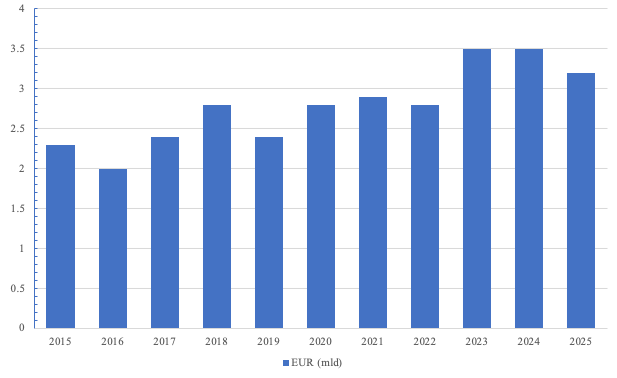
\includegraphics[height=6cm]{images/1_introduction/budget.png}
    \end{center}
    \caption{Budget for maintenance of public roads \cite{Rijksbegroting:Infrastructuur}. Budget is in billion (x1.000.000.000) EUR.}
    \label{fig:prm}
\end{figure}

Road maintenance is performed according to an annual cyclical process. The road owner or maintainer (i.e. state, province or municipality) initiates a tender for inspection. After which, an inspection company inspects the road with specialized vehicles. This vehicle contains of multiple cameras to record the road surface, infrared sensor to measure the evenness, and other types of sensors. The recorded video data is manually inspected by engineers according the prescribed CROW method \cite{CROW_147}. The inspection company delivers a report with recommendations to the road owner indicating which roads needs maintenance. On this recommendation, the road owner initiates another tender to perform the actual maintenance. Interestingly to note is that companies that can perform inspections, often also can perform the construction.

The condition of the road can thus measured through various quantifiable data sources. Below is a list given of data sources which are often used within the Netherlands for road inspection:
\begin{itemize}
\item Visual inspection: video data is manually annotated to mark damages.
\item ARAN measurements: laser sensor which measures distance between the road and vehicle across the pavement. This can be used to measure the surface unevenness or rutting.
\end{itemize}
\begin{itemize}
\item Ground penetrating radar: geophysical method which uses radar pulses to get an image of the subsurface by measuring the reflected signals. This enables to assess the quality of the asphalt and deeper layers, detect sinkholes and can detect objects below the surface.
\item Falling weight deflector: similar to ground penetrating radar, but instead of using radar pulses, a weight is dropped and reflections are measured. This method is more commonly used in civil engineering. 
\item Skid resistance: describes the force when a locked tire (i.e. a wheel that is prevented from rotating) slides along the surface. Measurements are performed by measuring the friction on the locked wheel. This method is used to detect if the road is too slippery e.g. aquaplaning.
\item Static data:  besides actual measurements, there is also static data available about roads.
\begin{itemize}
\item Materials passport describing the different layers of the road. Contains information when and how the layer was constructed and which material was used.
\item Historical maintenance reports.
\item Future date of maintenance (e.g. multi-year plan). 
\item Road intensity (how many vehicles travel the road).
\end{itemize}
    
\end{itemize}
Keeping track of these various sources of data is cumbersome. From experience it appears that  many road owners try to manage this data manually, that is without any specialized software. However, there are some tools in the industry to support their workflow. These software tools are known as "asset management software" or "management systems" . One of the available tools is Predictive Road Maintenance (PRM), a platform for data driven asset management (see figure \ref{fig:prm}). This tool is developed by AssetWorx \footnote{Pronounced as Asset Works}, this is also the startup where this thesis is written. PRM is created during an incubator program known as 'Startup in Residence' funded by the province Overijssel \cite{Residense2020}. As of now (Jul. 2021), PRM is only used by the province Overijssel, but AssetWorx is in active negotiation with other provinces and municipalities for adoption. The ultimate goal is to create an uniform data platform for road maintainers. The idea is to be a disrupter of the industry by providing data driven insights in road quality, maintenance and planning as an independent organization (i.e. not one of existing engineering firms). 

\begin{figure}[ht]
    \begin{center}
    \includegraphics[height=6cm]{images/1_introduction/prm-overview.png}
    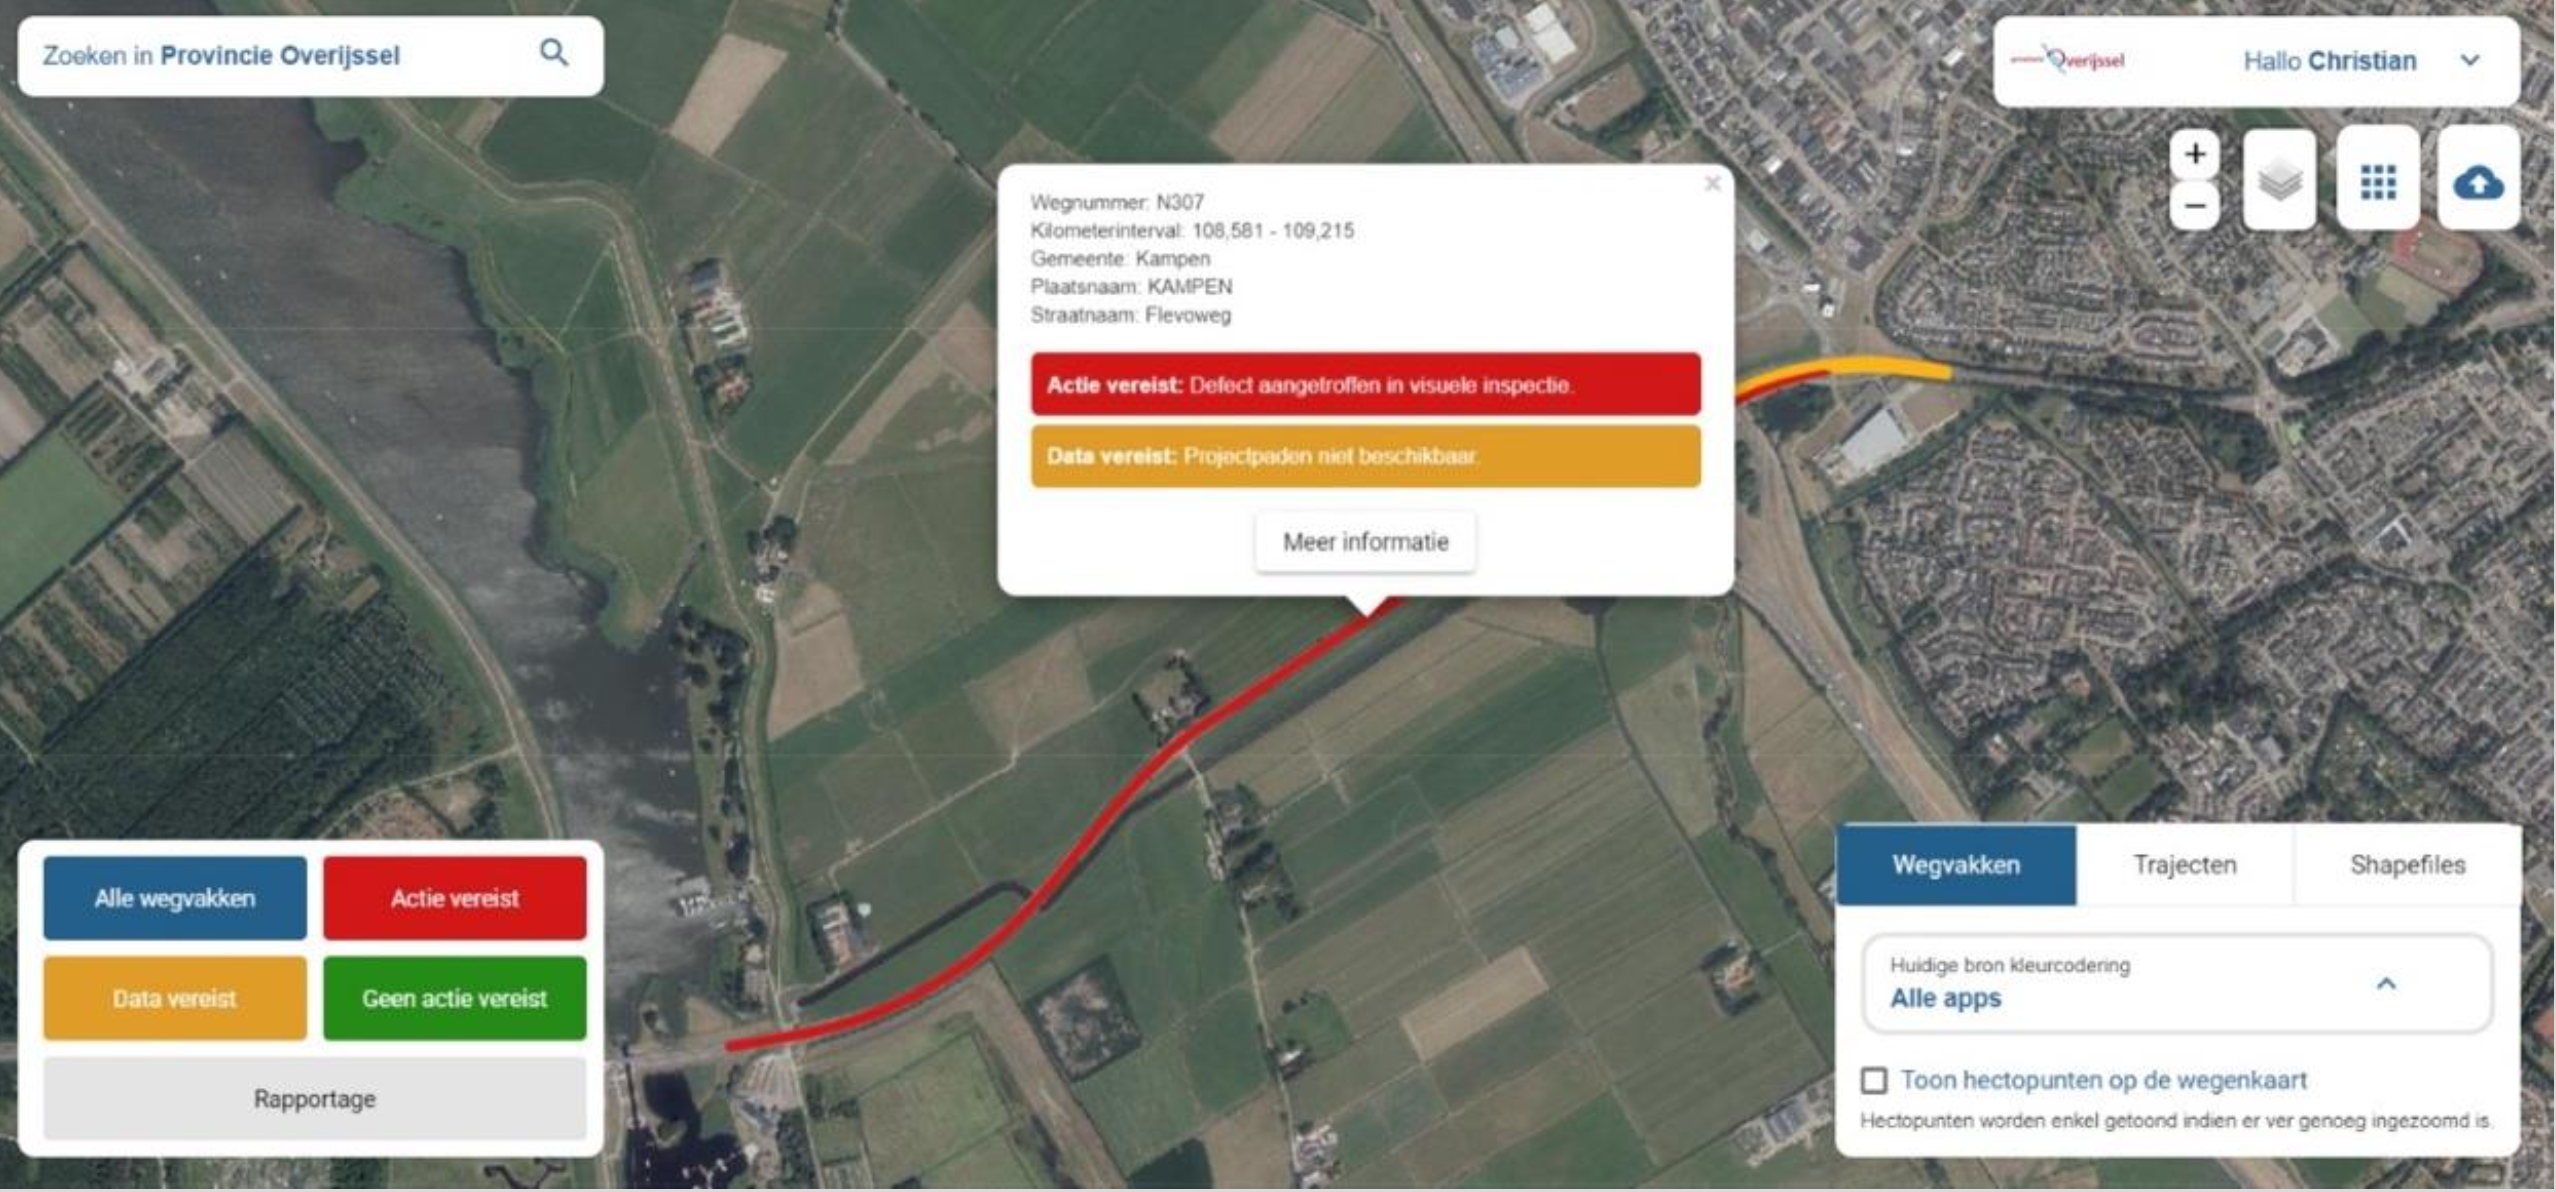
\includegraphics[height=6cm]{images/1_introduction/prm-detail.png}
    \end{center}
    \caption{Screenshots of Predictive Road Maintenance (PRM) software.}
    \label{fig:prm}
\end{figure}


\subsection{Relevance}

Although there are other asset management tools in the market, they typically only incorporate one or two data sources. PRM however is designed to operate on all kinds of data, as long the data can be geographically grounded (e.g. GPS coordinates). Currently, almost all road assessment rely on visual inspections based on the CROW systematic \cite{CROW_147}. This is an intensive procedure which largely relies on experience and intuition of the inspectors and maintainers. The cycle of tendering -> inspection -> tendering -> maintenance, typically takes one year. However, when there is a damage in the pavement, the severity of that damage may increase as it remains not repaired. For instance, a pothole starts relatively small but over time, as more traffic passes, it may become a significant damage in the road that eventually affects the drivers. Repairing a small pothole is easy and quick, but as the damages increases, so does the financial costs of repairing a road. Therefore, timely monitoring of road damages saves costs for the maintainer while increasing comfort of driving and safety.

AssetWorx aims to systematically and continuously collect data on roads instead of the conventional annual cycle of inspection and maintenance. Data is manually collected through a sensor box, more details follow in later section. The collected data is then processed to automatically determine the state of the road. In order to determine that state, research (in form of this thesis) is performed to automatically detect road surface damages. None of the existing management tools incorporate this functionality. From online articles, it seems that some construction companies try to pursue this for their own proprietary tools. Automatic detection of road surface defects thus yields a large business value for AssetWorx. When road defects can be detected in a short period, it means that repair costs are minimum, thus yielding a large societal value for road maintainers as well.

Although automatic defect detection have societal and business value, it is scientifically not something new. However, existing literature only utilizes a single source of data (unimodal) to detect damages. For this research, we are collecting various types of data: visual, sound, GPS, accelerations and the CAN bus. The CAN bus is the information bus used connecting different components within a car. Multimodal fusion aims to integrate data of different sources and types in a unified representation \cite{Baltrusaitis2017}. The idea is that by fusion richer information is provided than a single modality can provide. In order to scope the research, we will only be looking at fusing visual and accelerometer data. Within existing literature on road defects detection, multimodal fusion has not been applied. Additionally, fusion of accelerometer and visual data has only been researched in the context of odometry / robot navigation, not to detect damages or objects for that matter. Finally, fusion of visual and accelerometer data is an interesting challenge due time synchronization issue. As the image at timestamp $t_{visual}$ looks ahead, while the accelerometer measures the accelerations at some delay $t_{acc} = t_{visual} + \tau$. 


\subsection{Research Questions}


During this research we are collecting various types of data. To scope our research we only will be looking at fusing visual and accelerometer data. Reason for this is that these sources can be collected in the most reproducible way. The accelerometer is positioned at fixed point inside the vehicle, and a smartphone is attached to the windshield in a conventional holder. Although we also collect sounds and CAN-bus information, these sources are neglected for now. Road noise may not be reliable due conditions (radio, talking), and CAN-bus information differs for each vehicle.

Fusing these visual and accelerometer data is interesting. Visual data can only be recorded in good conditions (i.e. weather and lighting). Complementary, vibrations can always be measured regardless of external conditions. At the same time, interpreting vibration data might pose a difficult task for humans. Combining both data sources helps to interpret the data. With that in mind, this thesis aims to answer the following research question

\begin{itemize}
\item \textbf{RQ: How can we fuse visual and accelerometer data in an end-to-end multimodal deep learning model to classify road surface defects?}
\end{itemize}

In order to answer this question, we can divide it into smaller parts. First of all, to my knowledge, no research has been performed to use multimodal data for detecting road surface defects. However, there have been extensive research on uni-modal data (mostly based on images). To get a better understanding of this field, the first sub question is:

\begin{itemize}
\item \textit{SQ1: What kind of data and algorithms are used to detect road surface defects?}
\end{itemize}

The research is focused on fusing visual and vibration data. In order to fuse these data types, we need to make good representations on each respective data source. The visual data is most easily interpreted by humans. As road surface defects are basically objects in an image, the following research questions is formed:

\begin{itemize}
\item \textit{SQ2: What is state of the art in visual object detection?}
\end{itemize}

Although data fusion hasn't been used in detecting road surface defects, multimodal fusion has been used for visual and accelerometer data.

\begin{itemize}
\item \textit{SQ4: What is the state of the art in combining visual and sensor data for multimodal data fusion?}
\end{itemize}

Specifically we are interested in time synchronization to combine visual and vibration data. Since the camera records front-faced at timestamp $t_{visual}$, the vibration data at $t_{acc}$ is measured with some delay $\tau$. 

\begin{itemize}
\item \textit{SQ5: How to calculate the delay between front-faced visual data and the accelerations of the traveling vehicle?}
\end{itemize}


\subsection{Contributions}

TODO: Write out in actual words / alineas

Contributions of this thesis are as follows:
\begin{itemize}
\item Entrepreneur / social; 
\begin{itemize}
\item Automatic detection of road damages -> saves costs
\item Example data architecture of processing vehicle data on large scale
\end{itemize}
\item Scientific:
\begin{itemize}
\item Novel end-to-end model to detect road surface defects
\item Novel method to fuse future detected object with accelerometer data
\item Open-source code / data?
\end{itemize}
\end{itemize}



\subsection{Remainder}

The remainder of this thesis is structured as follows:

\begin{enumerate}
\addtocounter{enumi}{1}
\item \textbf{Literature} presents the current literature known on the subject. It answers the theoretical research subquestions 1-3. 
\item \textbf{Methodology} explains the methodology that is used during this thesis.
\item \textbf{Data Processing} presents the various data engineering activities required to record and process the data in order to make predictions.
\item \textbf{Multimodal Fusion} deals with the performed experiments.
\item \textbf{Discussion} interprets the results.
\item \textbf{Conclusion} concludes the thesis, and provides some suggestions for future activities.

\end{enumerate}

